\section{Funkce dvou reálných proměnných}

\begin{enumerate}

\item \textit{Reálna funkcia dvoch reálných premenných} $f:\mathbb{R}^2 \to \mathbb{R}$ je zobrazenie, ktoré každému $x \in \mathbb{R}^2$ priradí najviac jedno $f(x) \in \mathbb{R}$. \\
Prvky $x=[x_1,x_2]$ v $\mathbb{R}^2$ sa nazývajú body $2$-rozmerného priestoru $\mathbb{R}^2$, teda \textit{body v rovine}.  \\
Množina $\mathcal{D}(f)=\{x \in \mathbb{R}^2: \exists y \in \mathbb{R}: f(x)=y\}$ sa nazýva \textit{definičný obor funkcie $f$}.\\
Množina $\mathcal{H}(f)=\{y \in \mathbb{R}: \exists x \in \mathcal{D}(f): f(x)=y\}$ sa nazýva \textit{obor hodnôt funkcie $f$}.\\
Množina $\mathcal{G}(f)=\{[x_1,x_2] \in \mathbb{R}^2: [x_1,x_2] \in \mathcal{D}(f)\}$ sa nazýva \textit{graf funkcie $f$}.


\item Určite a načrtnite definičné obory nasledujúcich funkcií

\begin{enumerate}
\item[a)]{$u=x+\sqrt{y}$}\hspace{\fill}[Polrovina $y\geq0$]
\item[b)]{$u=\sqrt{1-x^2}+\sqrt{y^2-1}$}\hspace{\fill}[$|x|\leq 1$, $|y|\geq 1$]
\item[c)]{$u=\sqrt{1-x^2-y^2}$}\hspace{\fill}[Kruh $x^2+y^2 \leq 1$]
\item[d)]{$u=\frac{1}{\sqrt{x^2+y^2-1}}$}\hspace{\fill}[Vonkajšok kruhu $x^2+y^2>1$]
\item[e)]{$u=\sqrt{1-(x^2+y)^2}$}\hspace{\fill}[$-1\leq x^2+y \leq 1$]
\item[f)]{$u=\ln(-x-y)$}\hspace{\fill}[Polrovina $x+y < 0$]
\item[g)]{$u=\arcsin(\frac{y}{x})$}\hspace{\fill}[Dvojica uhlov $|y|<|x|$, $x\neq 0$]
\item[h)]{$u=\arcsin(\frac{x}{y^2})+\arcsin(1-y)$}\hspace{\fill}[Krivočiarý trojuholník vymedzený $y^2=x$, $y^2=-x$, $y=2$, $x \neq 0$]
\item[i)]{$u=\ln(xy)$}\hspace{\fill}[dva kvadranty priestoru]
\end{enumerate}

\item Zostrojte vrstevnice nasledujúcich funkcií

\begin{enumerate}
\item[a)]{$z=x+y$}\hspace{\fill}[Rovnobežné priamky]
\item[b)]{$z=x^2+y^2$}\hspace{\fill}[Sústredné kružnice]
\item[c)]{$z=x^2-y^2$}\hspace{\fill}[Množina hyperbol so spoločnými asymptotami $y=\pm x$]
\item[d)]{$z=(x+y)^2$}\hspace{\fill}[Rovnobežné priamky]
\item[e)]{$z=\frac{y}{x}$}\hspace{\fill}[Zväzok priamok s vrcholom v počiatku sústavy súradníc s vylúčením tohoto vrcholu]
\end{enumerate}

\item Buď $f:\mathbb{R}^2 \to \mathbb{R}$ reálna funkcia dvoch reálnych premenných, označme $K(x, \epsilon)=(x-\epsilon, x+\epsilon)$. Potom množina $\mathcal{D}(f)'=\{x \in \mathbb{R}^2: \forall \epsilon>0: (K(x,\epsilon)\setminus \{x\}) \cap \mathcal{D}(f) \neq \emptyset \}$ sa nazýva \textit{derivácia množiny $D(f)$.}

\item Povedzme, že $f$ má v bode $x_0 \in \mathcal{D}(f)'$ \textit{limitu} $a \in \mathbb{R}$ ak $\forall K(a,\epsilon)$ existuje $K(x_0,\delta)$ tak, že $\forall x \in (K(x,\epsilon) \setminus \{x_0\})\cap \mathcal{D}(f):f(x) \in K(a, \epsilon)=(a-\epsilon, a+\epsilon)$.

\item Vypočítajte nasledujúce limity

\begin{enumerate}
\item[a)]{$ \lim_{(x,y) \to (\infty,\infty)} \frac{x+y}{x^2-xy+y^2} $}\hspace{\fill}[0]
\item[b)]{$ \lim_{(x,y) \to (\infty,\infty)} \frac{x^2+y^2}{x^4+y^4} $}\hspace{\fill}[0]
\end{enumerate}

\item Nech $f:\mathbb{R}^2 \to \mathbb{R}$ je reálna funkcia dvoch premenných a $a=[a_1,a_2]$. Položme $f_1:\mathbb{R}\to \mathbb{R}$, $f_1(x_1)=f(x_1,a_2)$ a $f_2:\mathbb{R}\to \mathbb{R}$, $f_2(x_2)=f(a_1,x_2)$. \\
Číslo $f'_x(a):=f'_1(a_1)$ sa nazýva \textit{parciálna derivácia funkcie $f$ podľa $x$}. \\
Číslo $f'_y(a):=f'_2(a_2)$ sa nazýva \textit{parciálna derivácia funkcie $f$ podľa $y$}. 


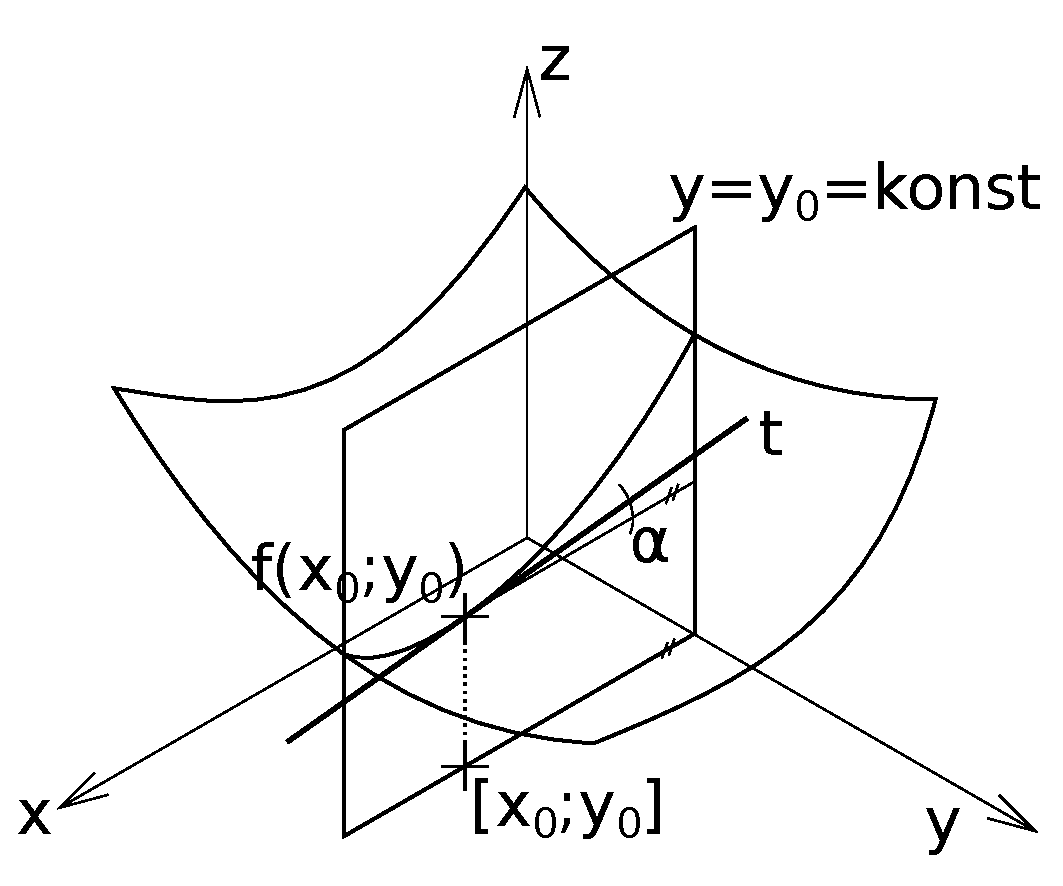
\includegraphics[scale=0.5]{Obrazky/ParcDer.pdf}

\item Vypočítajte parciálne derivácie prvého a druhého rádu u nasledujúcich funkcií
\begin{enumerate}
\item[a)]{$u=x^4+y^4-4x^2y^2$}\hspace{\fill}[$u'_{x}=4x^3-8xy^2$, $u'_y=4y^3-8x^2y$, $u''_{xx}=12x^2-8y^2$, $u''_{yy}=12y^2-8x^2$, $u''_{xy}=-16xy$]
\item[b)]{$u=xy+\frac{x}{y}$}\hspace{\fill}[$u'_{x}=y+\frac{1}{y}$, $u'_y=x-\frac{x}{y^2}$, $u''_{xx}=0$, $u''_{yy}=\frac{2x}{y^3}$, $u''_{xy}=1-\frac{1}{y^2}$]
\item[c)]{$u=\frac{x}{y^2}$}\hspace{\fill}[$u'_{x}=\frac{1}{y^2}$, $u'_y=-\frac{2x}{y^3}$, $u''_{xx}=0$, $u''_{yy}=\frac{6x}{y^4}$, $u''_{xy}=-\frac{2}{y^3}$]
\item[d)]{$u=\frac{x}{\sqrt{x^2+y^2}}$}\hspace{\fill}[$u'_{x}=\frac{y^2}{(x^2+y^2)^{\frac{3}{2}}}$, $u'_y=-\frac{xy}{(x^2+y^2)^{\frac{3}{2}}}$, $u''_{xx}=-\frac{3xy^2}{(x^2+y^2)^{\frac{5}{2}}}$, $u''_{yy}=-\frac{x(x^2-2y^2)}{(x^2+y^2)^{\frac{5}{2}}}$, $u''_{xy}=\frac{y(2x^2-y^2)}{(x^2+y^2)^{\frac{5}{2}}}$]
\item[e)]{$u=x\sin(x+y)$}\hspace{\fill}[$u'_x=\sin(x+y)+x\cos(x+y)$, $u'_y=x\cos(x+y)$, $u''_{xx}=2\cos(x+y)-x\sin(x+y)$, $u''_{xy}=\cos(x+y)-x\sin(x+y)$, $u''_{yy}=-x\sin(x+y)$]
\item[f)]{$u=\frac{\cos(x^2)}{y}$}\hspace{\fill}[$u'_x=\frac{2x\sin(x^2)}{y}$, $u'_y=-\frac{\cos(x^2)}{y^2}$, $u''_{xx}=-\frac{2\sin(x^2)+4x^2\cos(x^2)}{y}$, $u''_{xy}=\frac{2x\sin(x^2)}{y^2}$, $u''_{yy}=\frac{2\cos(x^2)}{y^3}$]
\item[g)]{$u=\tan(\frac{x^2}{y})$}\hspace{\fill}[$u'_x=\frac{2x}{y\cos^2(\frac{x^2}{y})}$, $u'_y=-\frac{x^2}{y^2\cos^2(\frac{x^2}{y})}$, $u''_{xx}=\frac{2}{y\cos^2(\frac{x^2}{y})}+\frac{8x^2\sin(\frac{x^2}{y})}{y^2\cos^3(\frac{x^2}{y})}$, $u''_{xy}=\frac{-2x}{y^2\cos^2(\frac{x^2}{y})}-\frac{4x^3}{y^3}\frac{\sin(\frac{x^2}{y})}{\cos^3(\frac{x^2}{y}}$, $u''_{yy}=\frac{2x^2}{y^3\cos^2(\frac{x^2}{y})}+\frac{2x^4}{y^4}\frac{\sin(\frac{x^2}{y})}{\cos^3(\frac{x^2}{y})}$]
\item[h)]{$u=x^y$}\hspace{\fill}[$u'_x=yx^{x-1}$, $u'_y=\ln(x)x^{y}$, $u''_{xx}=y(y-1)x^{y-2}$, $u''_{yy}=x^{y}\ln^2(x)$, $u''_{xy}=x^{y-1}(1+y\ln(x))$]
\item[i)]{$u=\ln(x+y^2)$}\hspace{\fill}[]
\item[j)]{$u=\arctan(\frac{x}{y})$}\hspace{\fill}[]
\end{enumerate}

\item Overte platnosť rovnice
$\frac{\partial^2 u}{\partial x \partial y}=\frac{\partial^2 u}{\partial y \partial x}$ pre funkcie u

\begin{enumerate}
\item[a)]{$u=x^2-2xy-3y^2$}
\item[b)]{$u=x^{y^2}$}
\end{enumerate}




\end{enumerate}